\documentclass[11pt,a4paper]{article}
\usepackage{{../../paquete-formulas}}
\usepackage{{../../estilos-formulas}}

\usepackage{array}
\newcolumntype{M}[1]{>{\centering\arraybackslash}m{#1}}%centrar en el medio y dar ancho a la columna del tabular
\newcommand{\materia}{Máquinas Eléctricas}

\begin{document}
	\pagestyle{pieyencabezado}
	\section*{Nomenclatura}
	
	\begin{tabular}{r l r l}
		$\fasor{Z}$ [$\Omega$]& Impedancia &
		$\fasor{i}$ [A] & Corriente \\
		$\fasor{v}$ [V] & Tensión&
		$j$ & Unidad imaginaria \\
		$t$ [s] & Tiempo &
		$P$ [W] & Potencia activa \\
		$Q$ [VAr] & Potencia reactiva &
		$\fasor{s}$ [VA] & Potencia aparente \\
		$m$ & Relación de transformación&
		$\fasor{I}_{exc}$ o $\fasor{I}_0$ [A] & Corriente de excitación\\
		$\fasor{I}_{Fe}$ [A] & Corriente debido a pérdidas en el Fe&
		$\fasor{I}_{\mu}$ [A] & Corriente magnetizante\\
		$\fasor{v}_0$ [V] & Tensión en vacío & $\fasor{v}_{pc}$ [V] & Tensión a plena carga \\
	\end{tabular}
	\unidad{1}{Acá quiero poner lo de las bobinas y eso... VER}
	
%	BEGIN_FOLD


	\unidad{2}{Transformadores}
	
	\begin{cajita}
		
		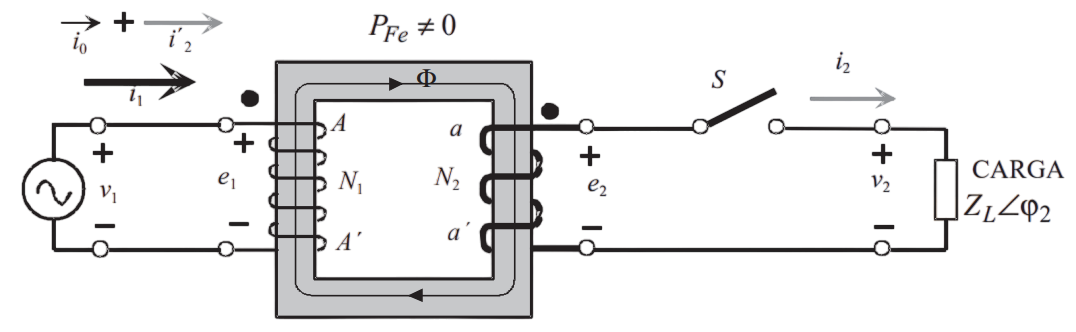
\includegraphics[width = .8\linewidth]{trafo-ideal}
		\begin{multicols}{2}
		
			\begin{center}
				\subtitulo{Transformador Ideal \textnormal{en vacío} \vspace{.1cm}} 
			\end{center}
			
			\subsubtitulo{sin pérdidas en el núcleo de Fe} 
			
			\begin{tabular}{l l}
				Autoinducción & $L = \dfrac{\mu N^2 S}{l}$ \\
			\end{tabular}
		
			\subsubtitulo{con pérdidas en el núcleo de Fe}
			
			\begin{tabular}{l l}
				Fem & $\mathcal{F} = N_1  \fasor{i}_1  = N_1  \fasor{i}_0$\\
				Relación de transfor. & $m = \dfrac{E_1}{E_2} = \dfrac{N_1}{N_2}$ \\
				\multicolumn{2}{c}{$ \fasor{i}_0 = \fasor{i}_\mu + \fasor{i}_{Fe} $} \vspace{.1cm} \\ 
				\multicolumn{2}{c}{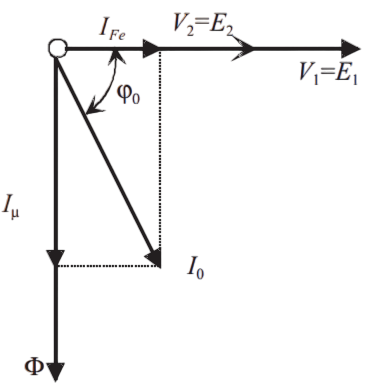
\includegraphics[width = .5\linewidth]{vacio-fasores}} \\
			\end{tabular} 
		
	
			\begin{center}
				\subtitulo{Transformador Ideal \textnormal{en carga}}
			\end{center}
		
			\vspace{-.6cm}
			
			\subsubtitulo{con pérdidas en el núcleo de Fe}
		
			\begin{tabular}{r l}
				Fem & $\mathcal{F} = N_1  \fasor{i}_1 - N_2 \fasor{i}_2$\\
				& $\mathcal{F} = N_1 \fasor{i}_0$\\
				& $\fasor{i}_0 = \fasor{i}_1 - \dfrac{N_2}{N_1} \fasor{i}_2$\\
				Corriente reducida & $\fasor{i'}_2 = \dfrac{\fasor{i}_2}{m}$ \\
			\end{tabular}
		
		\end{multicols}
	\end{cajita}
	\newpage
	\begin{cajita}
	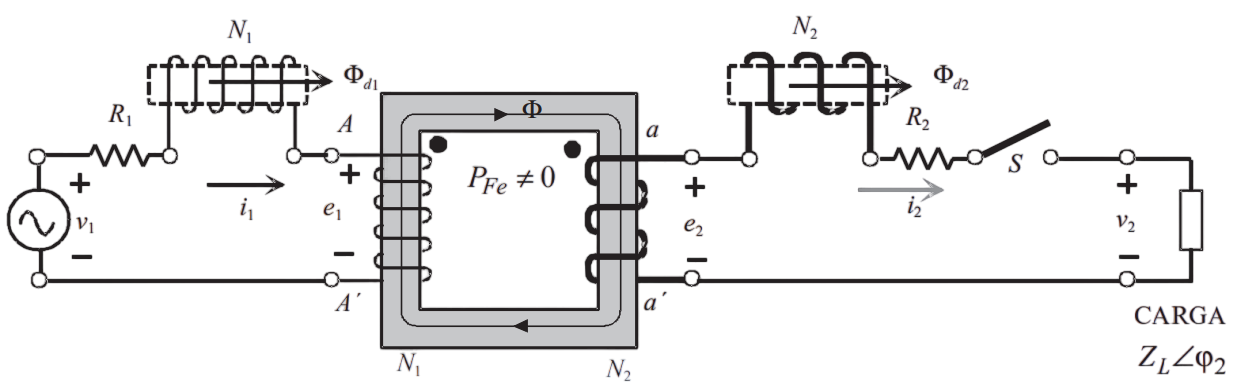
\includegraphics[width = .8\linewidth]{trafo-real}
	
	\begin{multicols}{2}
	
	\begin{center}
		\subtitulo{Transformador Real \textnormal{en vacío} \vspace{.1cm}}
	\end{center}
	
		\begin{tabular}{l l}
			$\fasor{v}_1 = \fasor{e}_1 + R_1 \fasor{i}_0 + j X_1 \fasor{i}_0$ & $\fasor{v}_{20} = \fasor{e}_2$ \\
			En trafos industriales & $m \approx \dfrac{V_1}{V_2}$\\
		\end{tabular}\\
	
		\begin{center}
			\subtitulo{Transformador Real \textnormal{en carga}}
		\end{center}		
		
	\end{multicols}
	\end{cajita}
	\begin{cajita}
	\subtitulo{Circuito equivalente aproximado}
	
	\begin{flushleft}
		Se muestra el circuito referido al primario. Cuando es referido al secundario se hace un análisis similar.
		
		La \textsl{rama paralelo} siempre permanece del lado de alta tensión.
	\end{flushleft}

	\begin{multicols}{2}
		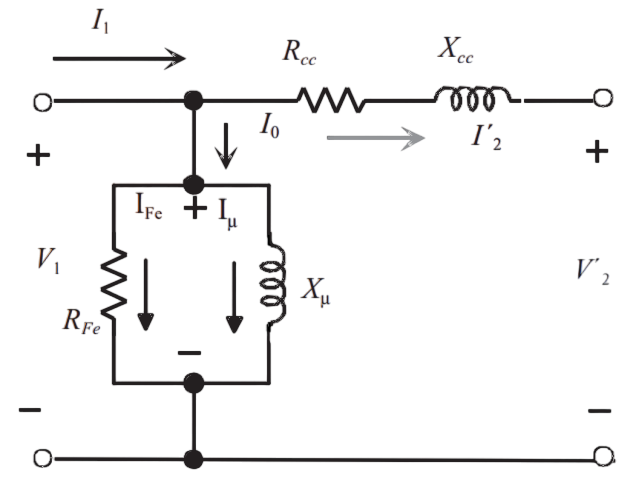
\includegraphics[width=.8\linewidth]{equi-aprox} \\
		
		\begin{tabular}{l l}
			Resistencia de cortocircuito &
			$R_{cc} = R_1 + R_2'$\\ \vspace{.1cm}
			Reactancia de cortocircuito & $X_{cc} = X_1 + X_2'$ \vspace{.2cm}  \\
			\multicolumn{2}{l}{\textbf{Parámetros referidos al primario} \vspace{.1cm}} \\ \vspace{.1cm}
			Número de espiras & $N_2' = m N_2$ \\ \vspace{.1cm}
			Tensión referida & $V_2' = m V_2$ \\ \vspace{.1cm}
			Corriente referida & $I_2' = \dfrac{I_2}{m}$ \\ \vspace{.1cm}
			Impedancia referida & $Z_2' = m^2 Z_2$ \\ \vspace{.1cm}
			& $Z_2 = R_2 + j X_2$\\
		\end{tabular}
	\end{multicols}
	\end{cajita}
	\begin{multicols}{2}
		\begin{cajita}
	\subtitulo{Ensayo de vacío}	
	
	
		\begin{flushleft}
			Permite determinar las pérdidas en el $Fe$
			y los parámetros de la rama paralelo, $R_{Fe}$ y $X_\mu$.
		\end{flushleft}
	
			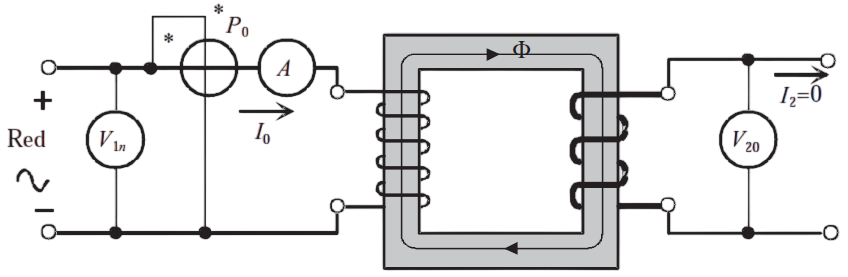
\includegraphics[width=\linewidth]{ensayo-vacio}\\ \vspace{.3cm}
			
			
			\begin{tabular}{c c}
					Pérdidas en Fe & $P_0 = P_{Fe} = V_{1n}\cdot I_0 \cos \phi_0$\vspace{.3cm} \\ 
					$ R_{fe}=\dfrac{V_{1n}}{I_{0} \cos \phi_0} $ &$X_{\mu}=\dfrac{V_{1n}}{I_{0}\sin \phi_0}$\\
			\end{tabular}\\
		
%			Se puede determinar la correspondencia entre las bobinas:\\
%			$\bullet$ A corresponde con y si: $V_{3}=V_{1}+V_{2}$\\
%			$\bullet$ A corresponde con x si: $V_{3}=V_{1}-V_{2}$\\
			
			\newpage %Similar al columnbreak pero deja alineado todo hacia arriba y no intenta distribuir en el eje y
		\end{cajita}	
	
	\begin{cajita}
	\subtitulo{Ensayo de cortocircuito}
		\begin{flushleft}
			Permite determinar las pérdidas en el $Cu$ y los parámetros de la rama de cortocircuito,  $R_{cc}$ y $X_{cc}$. $\fasor{I}_{0}$ es despreciable.
		\end{flushleft}
		
			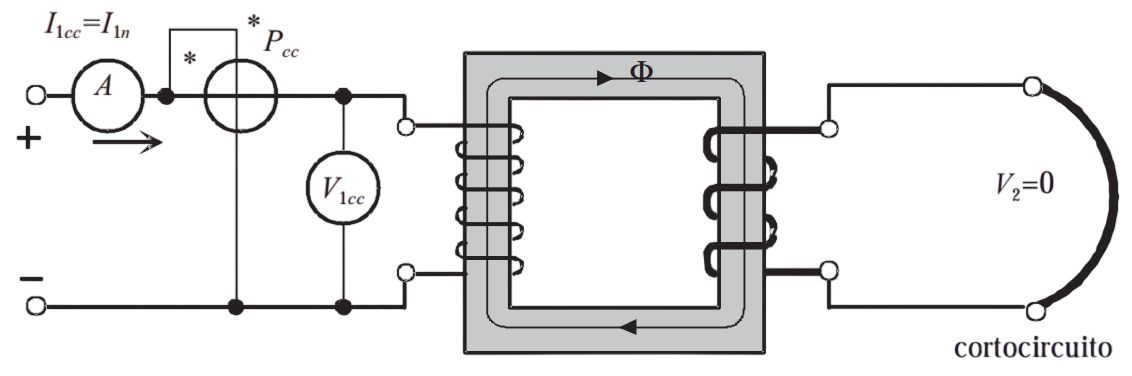
\includegraphics[width=\linewidth]{ensayo-cc}\\ \vspace{.1cm}
			
				
			\begin{tabular}{c c}
				\multicolumn{2}{c}{$P_{cc} = P_{Cu} =V_{cc}\cdot I_{1n} \cos\phi$}\\[0.1cm]
				$ R_{cc}=\dfrac{V_{1cc}}{I_{1n}} \cos\phi_{cc} $ &$X_{cc}=\dfrac{V_{1cc}}{I_{1n}} \sin\phi_{cc}$\\[0.4cm]
				
%							$\fasor{I}_{fe}=\fasor{I}_{0}.Cos[\phi_{0}] $& ; & $\fasor{I}_{\mu}=\fasor{I}_{0}.Sin[\phi_{0}] $\\[0.2cm]
			\end{tabular}
			\end{cajita}
	\end{multicols}
	En ambos ensayos, los factores de potencia $\cos \phi_{0}$ y $\cos \phi_{cc}$ son las incógnitas a determinar para calcular los parámetros.
	
		\begin{cajita}
		
		\subtitulo{Regulación de Voltaje}
		
		\begin{multicols}{2}
			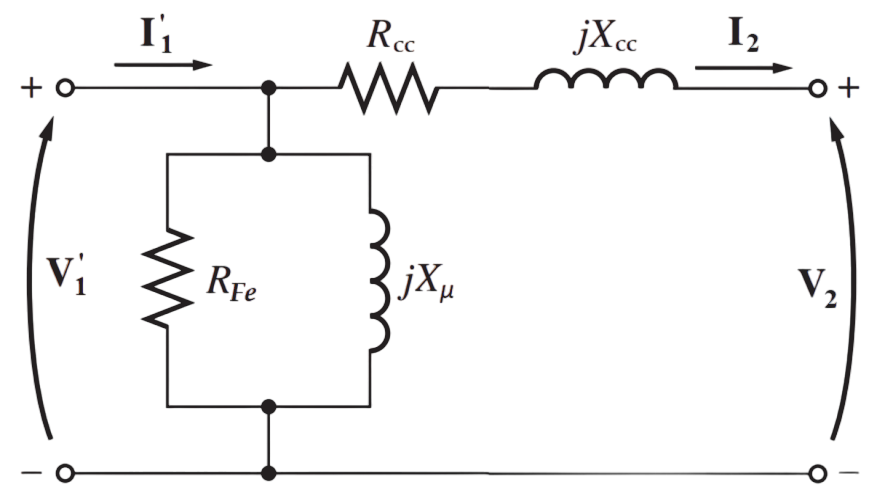
\includegraphics[width=\linewidth]{circuito-rv} \\
			
			\begin{tabular}{l l}
				Regulación de voltaje & $RV=\dfrac{V_{20}-V_{2pc}}{V_{2pc}}$\\[.3cm]
				& $RV = \dfrac{\frac{V_{1n}}{m} - V_{2pc}}{V_{2pc}}$\\[.3cm]
				RV ideal & $RV = 0 \%$ \\[.1cm]
				Cargas resistivas e inductivas & $RV_L > RV_R > 0$ \\[.1cm]
				Cargas capacitivas & $RV_C < 0$ \\
			\end{tabular}\\
		\end{multicols}
		
		\end{cajita}
		
		\begin{multicols}{2}
			\begin{cajita}
				\subtitulo{Eficiencia \vspace{.1cm}} 
				\vspace{.3cm}
				
				\begin{tabular}{l l}
					\multicolumn{2}{c}{$\eta = \dfrac{P_{out}}{P_{in}}= \dfrac{S \cos(\phi)}{S \cos(\phi )+P_{fe}+P_{\mu}}$\vspace{.2cm}}\\
					
%					Eficiencia máxima & $\cos\phi=1$ y $ P_{Fe}=P_{\mu }$ \\
					Potencia útil & $P_{out} = S \cos \phi$\\
					Potencia demandada & $P_{in} = P_{out} + P_{p}$\\
					Pérdidas en potencia & $P_p = P_{Fe} + P_\mu$\\
				\end{tabular}
			\end{cajita}
			
			\begin{cajita}
				\subtitulo{Índice de Carga}
				\vspace{.3cm}
				
				\begin{tabular}{l l}
					$C = \dfrac{I}{I_n}$ & $C_{opt} = \sqrt{\dfrac{P_0}{P_{cc}}}$\\
				\end{tabular}
			\end{cajita}
			\begin{cajita}
				\subtitulo{Máximo maximorum}\vspace{.3cm}
				Cuando $\cos\phi=1$ y $C_{opt} = \sqrt{\dfrac{P_0}{P_{cc}}}$.
			\end{cajita}
		\end{multicols}
	\begin{cajita}
		\subtitulo{Transformadores trifásicos}\vspace{.5cm}
		
			\begin{tabular}{| M{1.5cm} | M{1.5cm} | M{1.5cm}  M{1.5cm} | M{1.5cm} | M{1.5cm} | M{1.5cm}  M{1.5cm} |}
				\hline
			 & & \multicolumn{2}{c|}{Diagrama fasorial} & & & \multicolumn{2}{c|}{Diagrama fasorial}  \\
			 \multirow{-2}{1.5cm}{\centering Índice horario} & \multirow{-2}{1.5cm}{\centering Símbolo acoplam.} & A.T. & B.T. & \multirow{-2}{1.5cm}{\centering Índice horario} & \multirow{-2}{1.5cm}{\centering Símbolo acoplam.} & A.T. & B.T. \\
			 \hline
			0 ($0^\circ$)   & Dd0 & 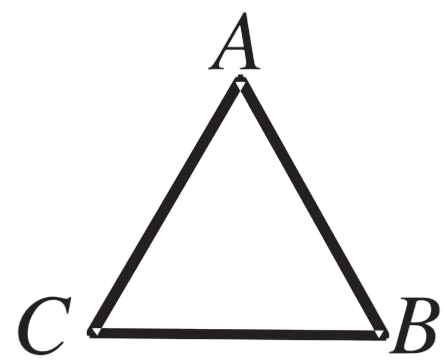
\includegraphics[height=1.2cm]{trianguloabc} & 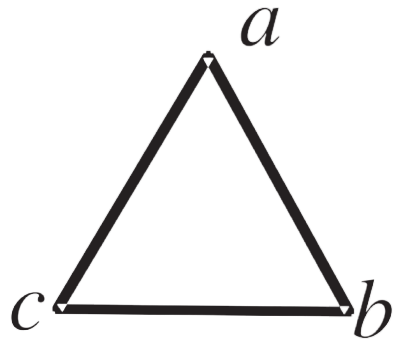
\includegraphics[height=1.2cm]{dd0bt} & 6 ($180^\circ$) & Dd6 & 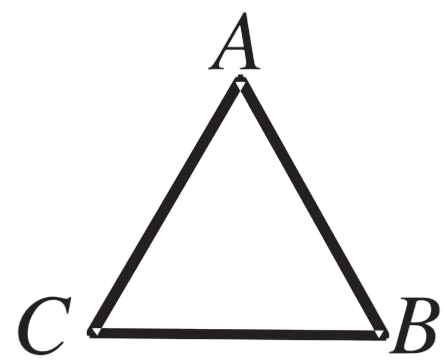
\includegraphics[height=1.2cm]{trianguloabc} & 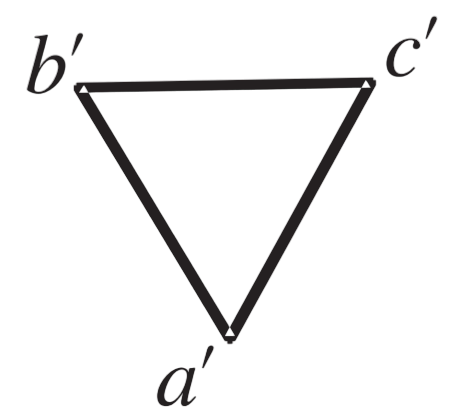
\includegraphics[height=1.2cm]{dd6bt}\\
			0 ($0^\circ$)   & Yy0 & 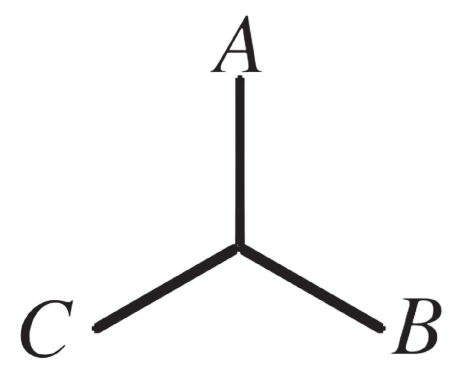
\includegraphics[height=1.2cm]{estrellaabc} & 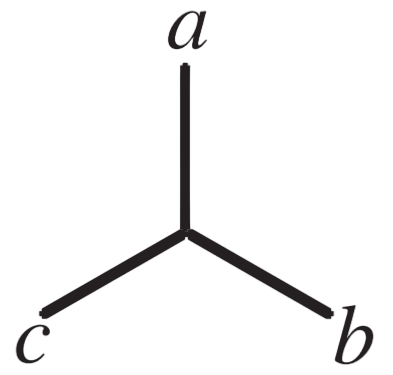
\includegraphics[height=1.2cm]{yy0bt} & 6 ($180^\circ$) & Yy5 & 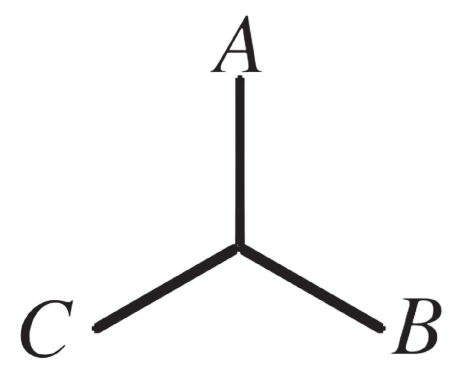
\includegraphics[height=1.2cm]{estrellaabc} & 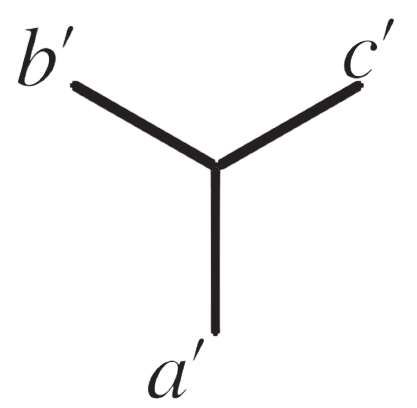
\includegraphics[height=1.2cm]{yy6bt} \\ \hline
			5 ($150^\circ$) & Dy5 & 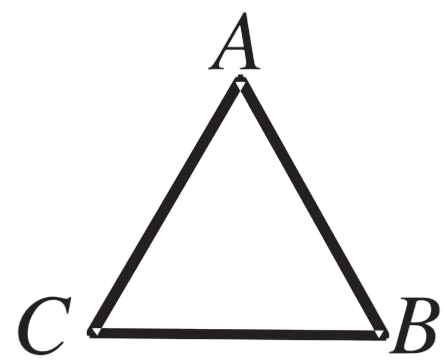
\includegraphics[height=1.2cm]{trianguloabc} & 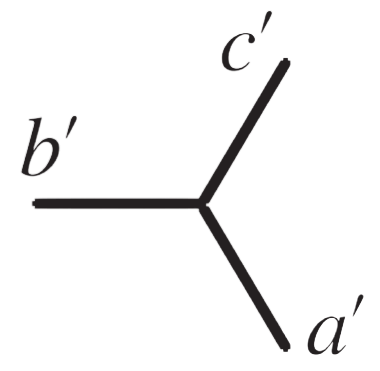
\includegraphics[height=1.2cm]{dy5bt} & 11 ($330^\circ$) & Dy5 & 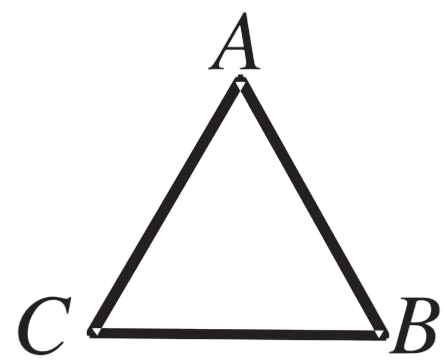
\includegraphics[height=1.2cm]{trianguloabc} & 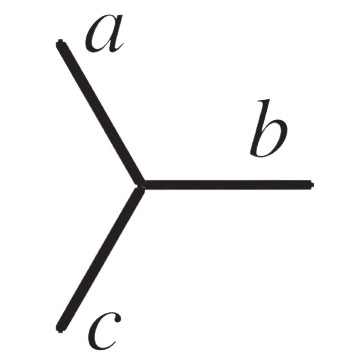
\includegraphics[height=1.2cm]{dy11bt} \\
			5 ($150^\circ$) & Yd5 & 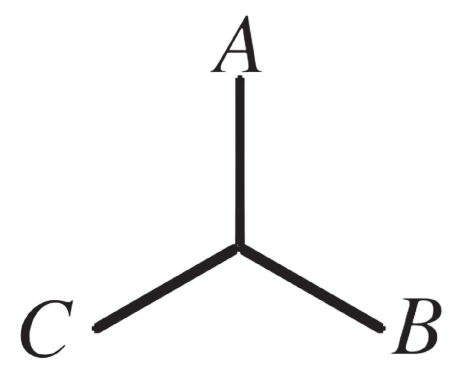
\includegraphics[height=1.2cm]{estrellaabc} & 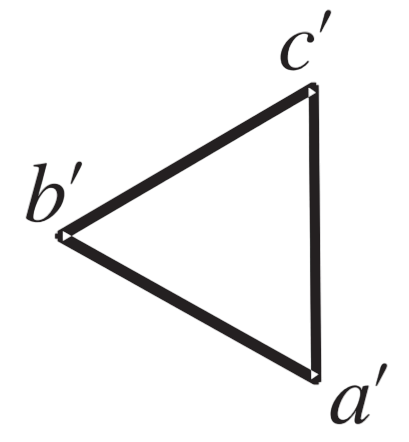
\includegraphics[height=1.2cm]{yd5bt} & 11 ($330^\circ$) & Yd5 & 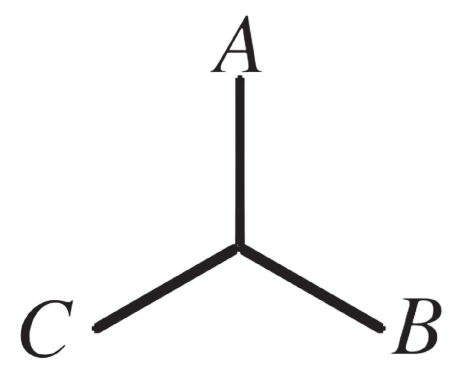
\includegraphics[height=1.2cm]{estrellaabc} & 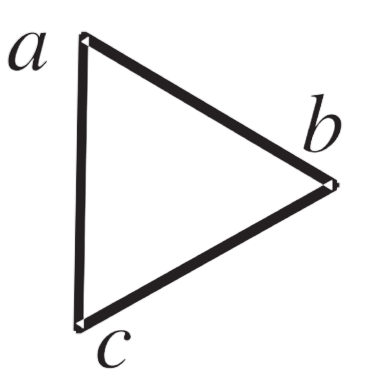
\includegraphics[height=1.2cm]{yd11bt} \\ \hline
			
			
			
			
		\end{tabular}
	
	\end{cajita}
%	END_FOLD

	\newpage
%	BEGIN_FOLD
	\unidad{3}{Máquinas asíncronas}
	\begin{cajita}
		\subtitulo{Aspectos básicos}
		\begin{multicols}{2}
			\begin{tabular}{l l}
				Tension inducida & $e_{ind} = l \vec{v} \times \vec{B}$\\
				Fuerza en el devanado & $F = i \vec{l} \times \vec{B}$\\
				\multicolumn{2}{l}{l es la longitud del segmento y su dirección es la de la corriente}\\ \vspace{.1cm}
				Velocidad campo rotante & $n_{sinc} = \dfrac{120}{P} f_{e}$\\
				Deslizamiento & $ s = \dfrac{n_{sinc} - n_{m}}{n_{sinc}} = \dfrac{\omega_{sinc} - \omega_{m}}{\omega_{sinc}}$\\
				Frecuencia eléctrica en el rotor & $f_{r} = s f_{e}$
			\end{tabular}
		\end{multicols}
	\end{cajita}
	
	\begin{cajita}
		\subtitulo{Circuito equivalente}
		\begin{multicols}{2}
			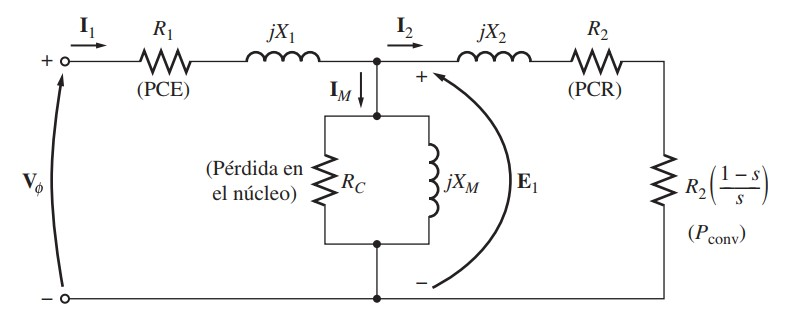
\includegraphics[width= .9\linewidth]{U3-Circuito_equivalente}\\ \vspace{.1cm}
			\begin{gather*}
					R_{2} = a_{ef}^{2} R_{R}\\
				X_{2} = a_{ef}^{2} X_{R0}\\
				E_{2} = a_{ef} E_{R0}\\
				I_{2} = \dfrac{I_{R}}{a_{ef}}			
			\end{gather*}
		\end{multicols}
		Donde el subíndice \emph{R0} equivale a los parámetros a rotor bloqueado, es decir s=1
	\end{cajita}
	
	\begin{cajita}
		\subtitulo{Diagrama de potencias}
		\begin{multicols}{2}
					\vspace{.5cm}
				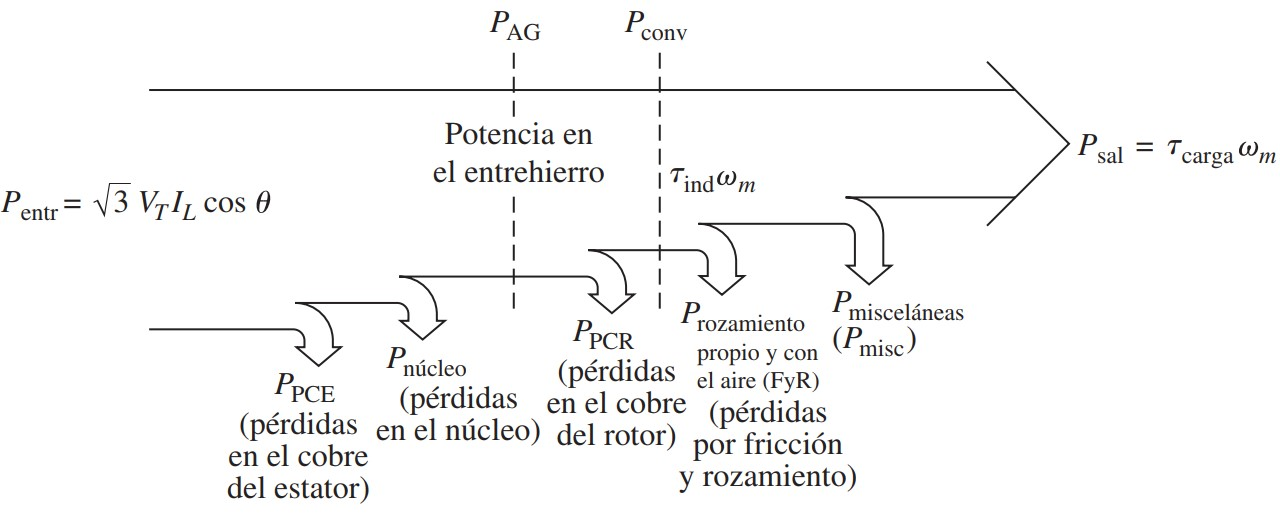
\includegraphics[width = \linewidth]{U3-Diagrama-potencia} \\
				\begin{center}
					\begin{tabular}{r l}
						\vspace{.2cm}
						Perdidas cobre estator & $P_{CE} = 3 I_{1}^{2} R_{1}$\\ \vspace{.2cm}
						Pérdidas en el núcleo & $P_{nucl} = 3 E_{1}^{2} G_{C}$\\ \vspace{.2cm}
						Potencia en el entrehierro & $P_{EH} = P_{in} - P_{CE} - P_{nucl}$\\ \vspace{.2cm}
						Pérdidas cobre rotor & $P_{CR} = 3 I_{2}^{2} R_{2}$\\ \vspace{.2cm}
						Potencia convertida & $P_{conv} = P_{EH} - P_{CR}$\\ \vspace{.2cm}
						$P_{CR} = s P_{EH}$ & $P_{conv} = (1-s) P_{EH}$\\ \vspace{.2cm}
						Potencia de salida & $P_{out} = P_{conv} - P_{FyR} - P_{misc}$ \\ 
						\multicolumn{2}{c}{$\tau_{ind} = \dfrac{P_{conv}}{\omega_{m}} = \dfrac{(1-s) P_{EH}}{(1-s) \omega_{sinc}}$}						
					\end{tabular}
				\end{center}
		\end{multicols}
	\end{cajita}
	
	\begin{cajita}
		\subtitulo{Ensayos de motor asincrónico}
	\end{cajita}
%	END_FOLD

\end{document}